%!TEX root = report.tex

\chapter{Anhang} % (fold)
\label{cha:anhang}

\section{Codebeispiel} % (fold)
\label{sec:codebeispiel}
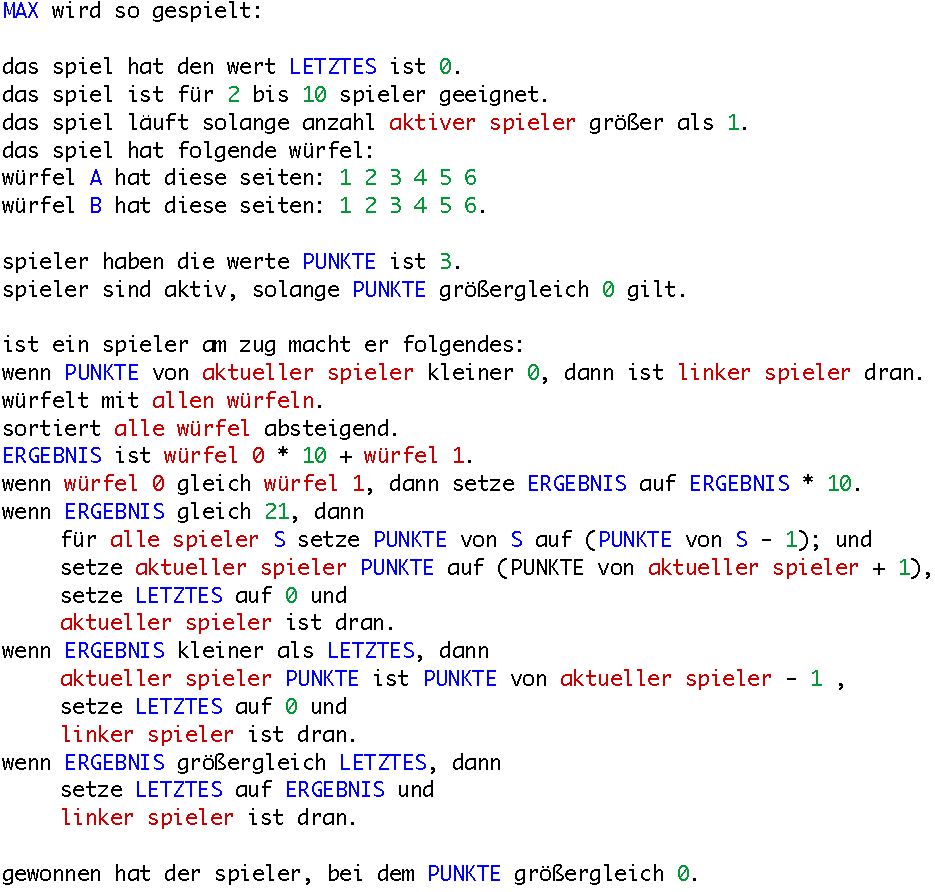
\includegraphics[width=0.9\textwidth]{example-code-crop.pdf}
\newpage
% section codebeispiel (end)
\section{Generierter Code} % (fold)
\label{sec:generierter_code}
\begin{lstlisting}[language=Python]
#!/usr/bin/env python
# -*- coding: utf-8 -*-
import random

class Player:
    def __str__(self): return self.name + ', ' + ', '.join(map(str, [value for key, value in self.__dict__.items() if key not in ['name']]))
    def __init__(self, name): self.name = name; self.PUNKTE = 3; 
    def isActive(self): return self.PUNKTE >= 0; 

class Dice:
    def __init__(self, name, faces): self.name = name; self.faces = faces; self.roll()
    def roll(self): self.value = random.choice(self.faces)
    def __str__(self): return self.name+': '+str(self.value)
class Game:
    # Static methods
    def status(self): return 'Status[name, ' + ', '.join([key for key, value in self.players[0].__dict__.items() if key not in ['name']]).lower()+']: '+' - '.join(map(str, self.players))
    def rightPlayer(self): return self.players[ (self.players.index(self.activePlayer) - 1) % self.playerCount]
    def leftPlayer(self):  return self.players[ (self.players.index(self.activePlayer) + 1) % self.playerCount]
    def playerNum (self, num): return self.players[num]
    def rollDices(self): map(Dice.roll, self.dices)
    def sortDices(self, desc=False): self.dices = sorted(self.dices, key=lambda dice: dice.value, reverse=desc)
    def setup(self):
        self.playerCount = int(raw_input('Enter number of players: '))
        if self.playerCount < self.min: print(self.name+' is made for more than '+str(self.min)+' players. Bring some friends ;-)'); exit()
        if self.playerCount > self.max: print(str(self.playerCount)+' players? Thats too much for '+self.name+'... Maximum: '+str(self.max)); exit()
        
        for p in range(self.playerCount): name = raw_input('Enter name of player #'+str(p)+': '); self.players.append(Player(name))
        self.activePlayer = self.players[0]
        print('Game initialized '+self.status())
        
    def isRunning(self): return (len([aktiver spieler, aktiver spieler]) > 1)
    def __init__(self):
        self.players = []
        # Dynamic inits
        self.name = 'MAXCHEN'
        
        self.LETZTES = 0
        self.min = 2
        self.max = 10
        self.dices = [Dice('A',[1, 2, 3, 4, 5, 6, ]), Dice('B',[1, 2, 3, 4, 5, 6, ]), ]
    def loop(self):
        while self.isRunning():   
            print(self.status())
            print('\n'+self.activePlayer.name+' ist dran.'),
            
            if self.activePlayer.PUNKTE < 0:
                self.activePlayer = self.leftPlayer(); continue
            raw_input('Enter drücken zum Würfeln...'); map(Dice.roll, self.dices); print('Du hast '+', '.join(map(str, [dice.value for dice in self.dices]))+' gewürfelt!')
            self.sortDices(desc=True)
            self.ERGEBNIS = self.dices[0].value * 10 + self.dices[1].value
            if self.dices[0].value == self.dices[1].value:
                self.ERGEBNIS = self.ERGEBNIS * 10
            if self.ERGEBNIS == 21:
                for self.S in self.players:
                    self.S.PUNKTE = (self.S.PUNKTE - 1)
                
                self.activePlayer.PUNKTE = (self.activePlayer.PUNKTE + 1)
                self.LETZTES = 0
                self.activePlayer = self.activePlayer; continue
            if self.ERGEBNIS < self.LETZTES:
                self.activePlayer.PUNKTE = self.activePlayer.PUNKTE - 1
                self.LETZTES = 0
                self.activePlayer = self.leftPlayer(); continue
            if self.ERGEBNIS >= self.LETZTES:
                self.LETZTES = self.ERGEBNIS
                self.activePlayer = self.leftPlayer(); continue

if __name__ == '__main__':
    game = Game()
    game.setup()
    game.loop()
    print('\nSpiel beendet: '+game.status())
    print([self.name for self in game.players if self.PUNKTE >= 0][0]+' hat gewonnen!')
\end{lstlisting}
% section generierter_code (end)

\section{Abstrakte Syntax} % (fold)
\label{sec:abstrakte_syntax}
\begin{center}
    \makebox[\textwidth][c]{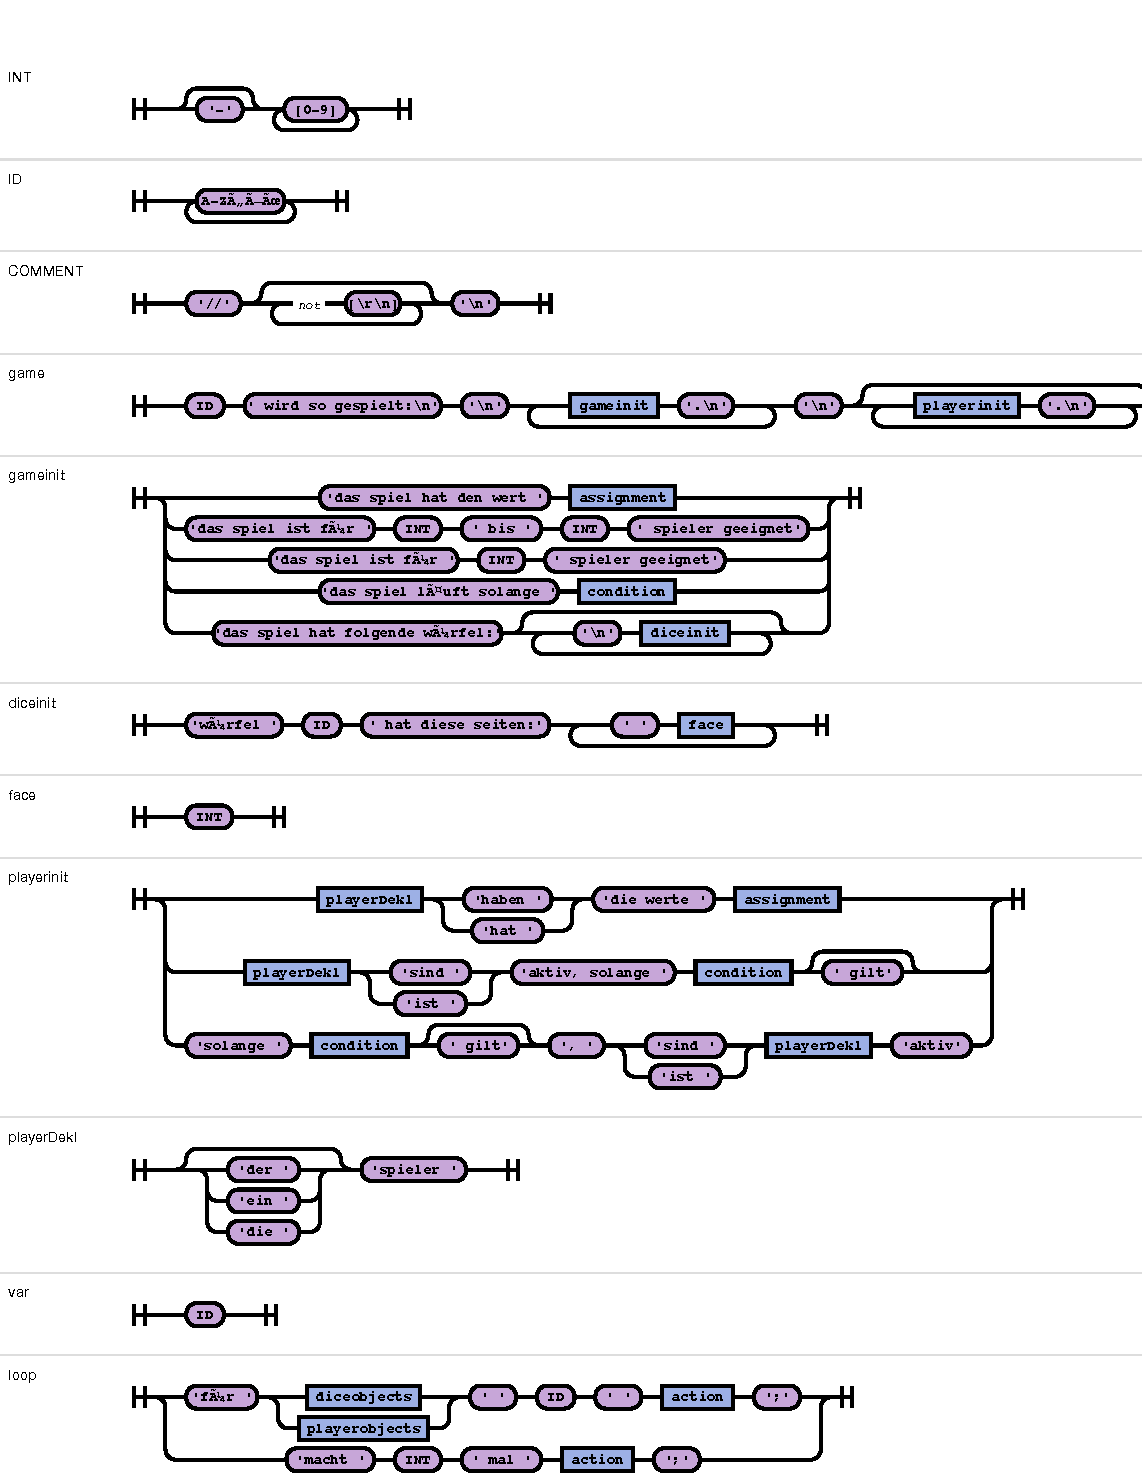
\includegraphics[width=1.1\textwidth]{ASG1-crop.pdf}}~\newpage
    \makebox[\textwidth][c]{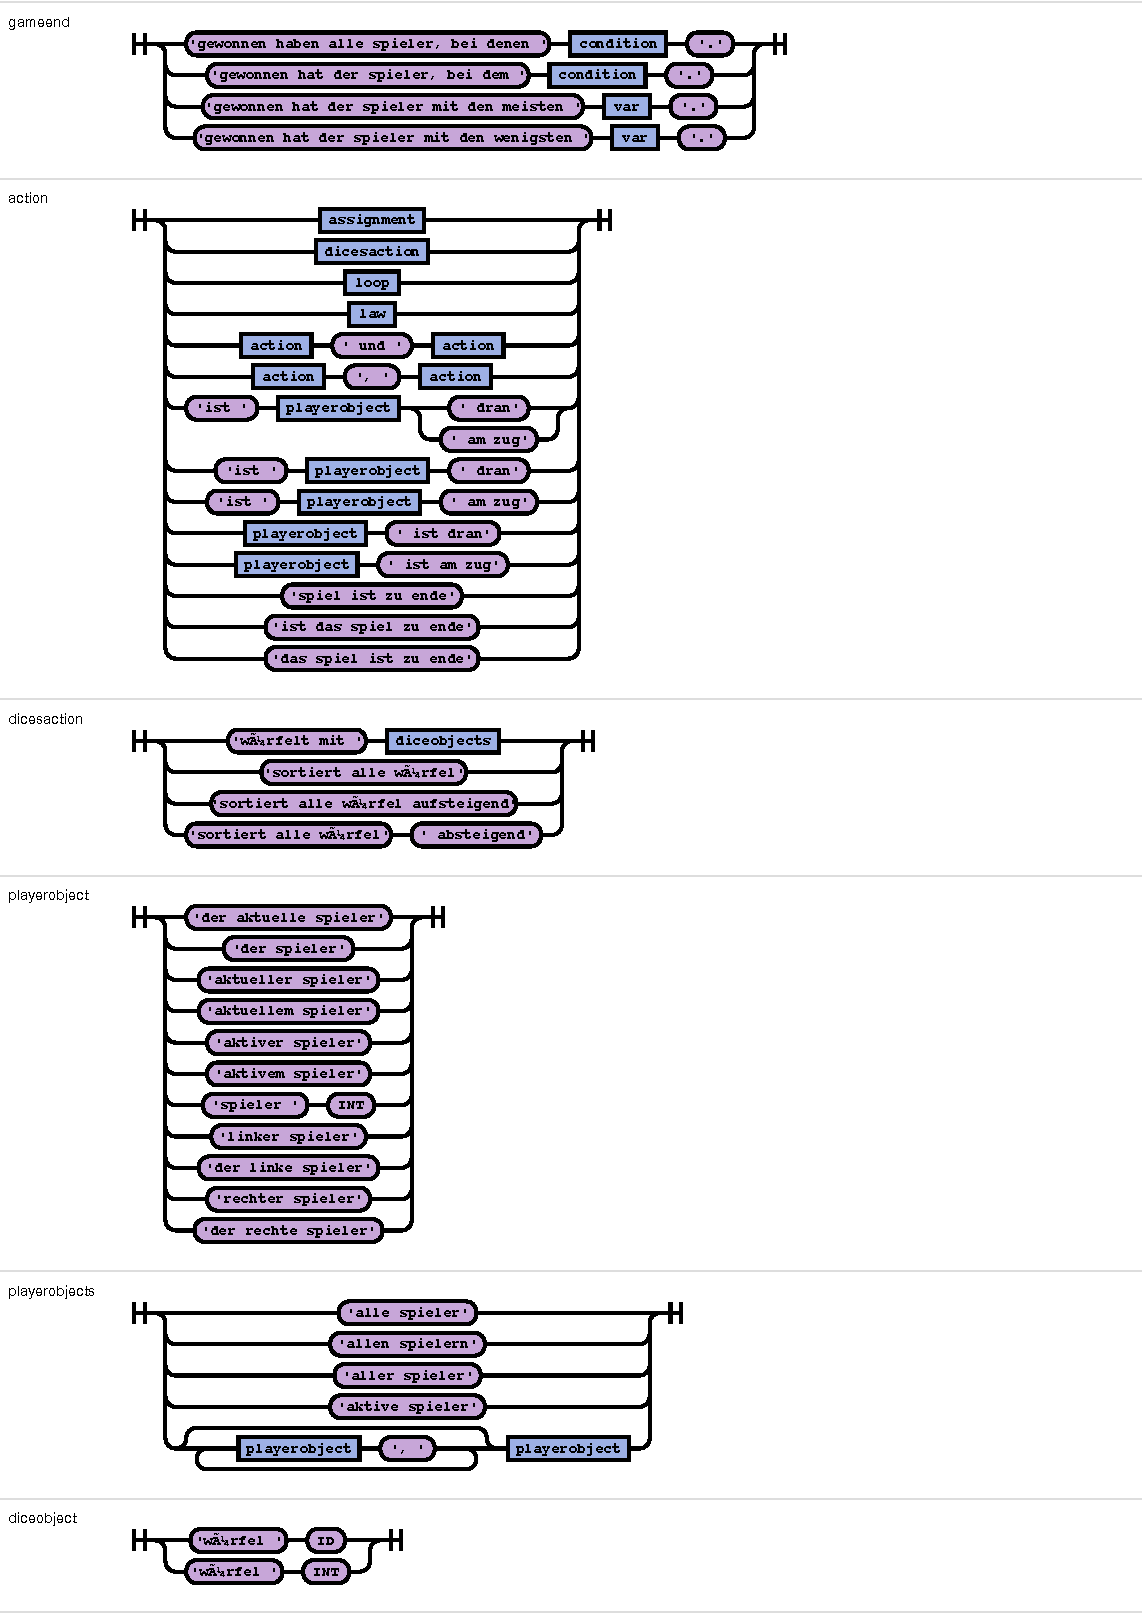
\includegraphics[width=1.1\textwidth]{ASG2-crop.pdf}}~\newpage
    \makebox[\textwidth][c]{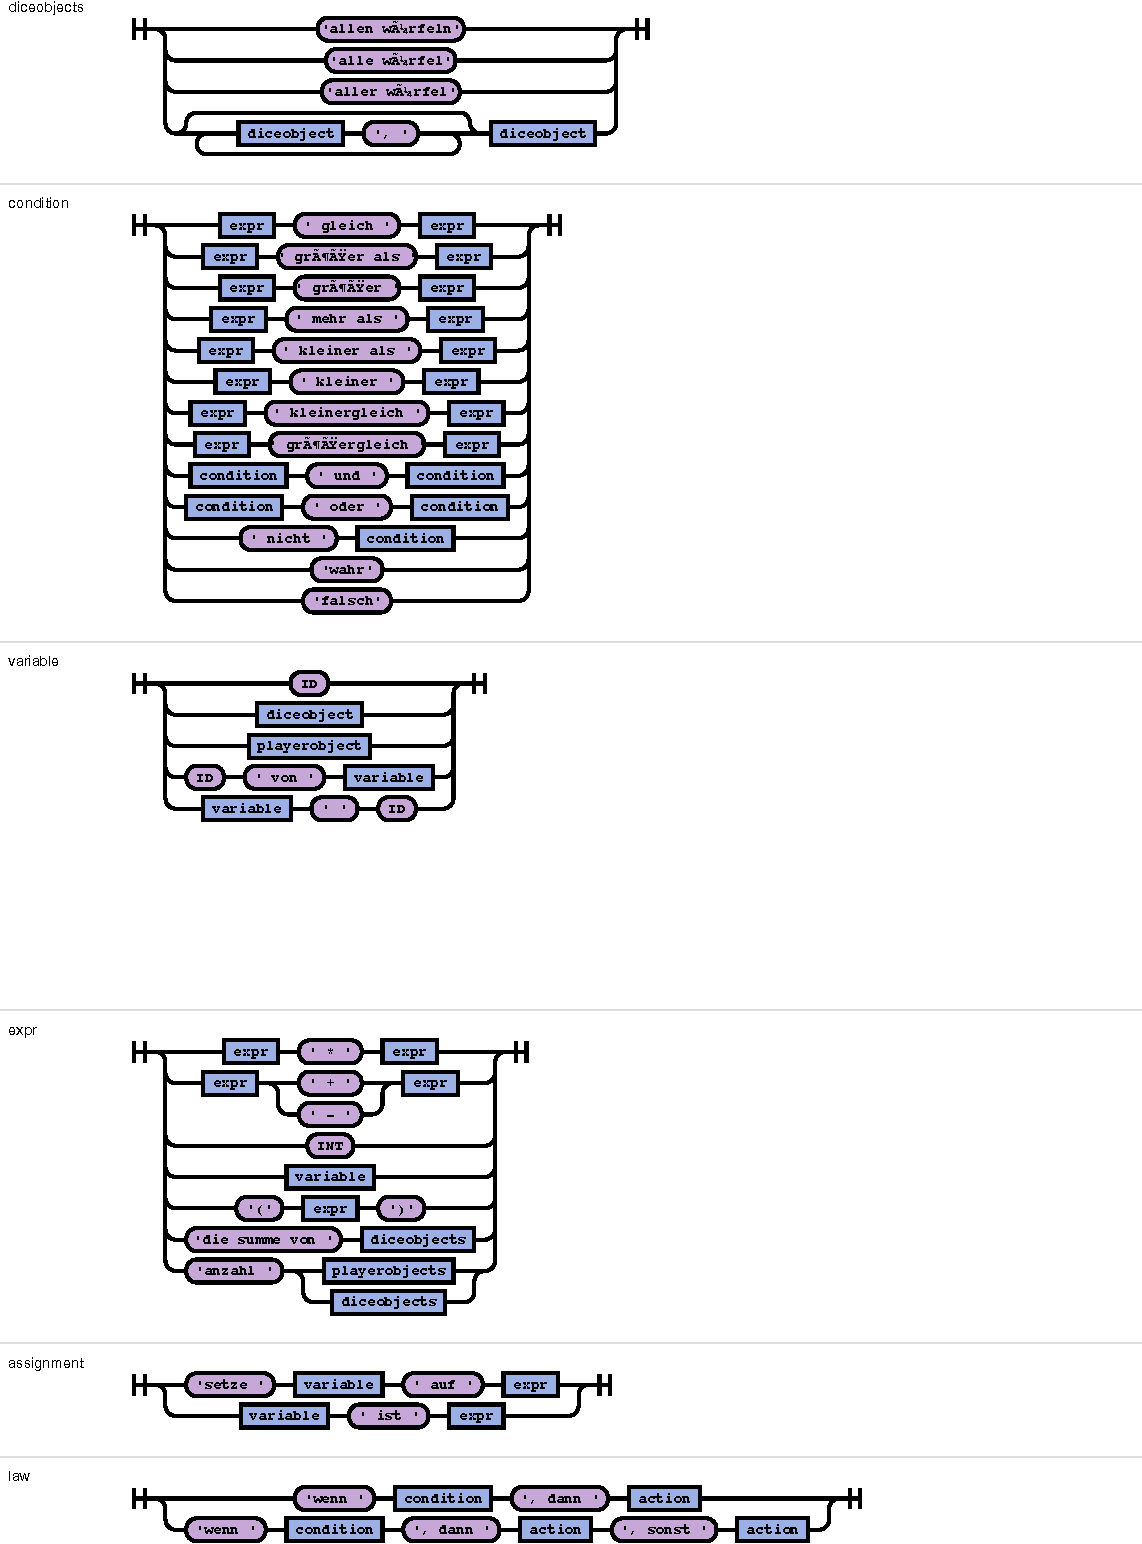
\includegraphics[width=1.1\textwidth]{ASG3-crop.pdf}}
\end{center}
% section abstrakte_syntax (end)
% chapter anhang (end)